\documentclass[a4paper,12pt]{article}
\usepackage{geometry}
\geometry{left=2cm}
\geometry{right=1.5cm}
\geometry{top=3cm}
\geometry{bottom=3cm}

\usepackage[unicode=true, colorlinks=false, hidelinks]{hyperref}
\usepackage[utf8]{inputenc}
\usepackage[english, russian]{babel}
\usepackage{mathtext}
\usepackage[T2A, TS1]{fontenc}
\usepackage{microtype} % Slightly tweak font spacing for aesthetics
\usepackage{amsthm, amssymb, amsmath, amsfonts, nccmath}
\usepackage{nicefrac}
\usepackage{epstopdf}
\usepackage[export]{adjustbox}
\usepackage{float} % Improved interface for floating objects
\usepackage{graphicx, multicol} % Enhanced support for graphics
\usepackage{pdfrender,xcolor}

\usepackage{mathtools}
\usepackage{titling}
\usepackage{bm}
\usepackage{centernot}
\usepackage[cal=boondoxo,calscaled=.96]{mathalpha}
\usepackage{marvosym, wasysym} % More symbols
\usepackage{rotating} % Rotation tools
\usepackage{censor} % Facilities for controlling restricted text
\usepackage{indentfirst}
\usepackage{svg}

\DeclareMathOperator{\cov}{cov}
\DeclareMathOperator{\med}{med}
\DeclareMathOperator{\sign}{sign}

\usepackage{array}
\newcolumntype{C}[1]{>{\centering\let\newline\\\arraybackslash\hspace{0pt}}m{#1}}

\usepackage{fancyhdr}
\pagestyle{fancy}
\fancyhead{}\renewcommand{\headrulewidth}{0pt}
\fancyfoot[L]{}
\fancyhead{}
\fancyfoot{}
\fancyfoot[R]{\thepage}
\begin{document}
\begin{titlepage}
	\newpage
	
	\begin{center}
		\textrm{\large Санкт-Петербургский политехнический университет \linebreak Петра Великого \\}
	\end{center}
	
	\begin{center}
			\textrm{\large Физико-механический институт \\ Высшая школа прикладной математики и физики \\}
	\end{center}

	\vspace{10em}
	
	\begin{center}
		\textrm{\textbf{\large Отчёт \linebreak по дополнению к лабораторной работе №4 \\
				по дисциплине \\ «Интервальный анализ»}}
	\end{center}
	
	\vspace{8em}
	
	\hfill\parbox{11cm}{
		\hspace*{4cm}Выполнил студент: \\
		\hspace*{4cm}Чевыкалов Г.А. \\
		\hspace*{4cm}Группа: 5030102/90201 \\
		\hspace*{4cm}Проверил: \\
		\hspace*{4cm}к.ф.-м.н., доцент \\
		\hspace*{4cm}Баженов Александр Николаевич \\
	}
	
	
	\vspace{\fill}
	
	\begin{center}
		Санкт-Петербург \\ 2022
	\end{center}
	
\end{titlepage}
\newpage
\tableofcontents
\newpage
\listoffigures
\newpage
\section{Постановка задачи}
Дан набор интервальных данных. Необходимо исключить из рассмотрения данные, у которых координата $x$ не принадлежит промежутку $[50, 150]$. Считая что они задают линейно распределенную величину, требуется построить информационное множество параметров, корридор совместности и произвести "предсказание значений": 
\begin{itemize}
    \item 1 - для значения между имеющимися данными (интерполяция).
    \item 2 - для значений вне имеющихся данных (экстраполяция).
\end{itemize}
Сравнить реальные значения с полученной оценкой.
\section{Теория}
\subsection{Точечная оценка параметров регрессии}
     Пусть $x$ - номер измерения в выборке, а $y$ - получившийся результат. Тогда мы можем представить линейную регрессию как
     $$ y = b_0 + b_1 * x$$
     Для получения точечной оценки можно поставить задачу оптимизации
     \begin{equation}
        \begin{cases}
            $$mid(y_i) - w_i * rad(y_i) \le X *\beta \le mid(y_i) + w_i * rad(y_i)$$ & i=1,m\\
            $$\sum_{i = 1}^m w_i -> min$$ \\
            $$w_i \ge 0$$ & i = 1,m \\
            $$w, \beta = ?$$
        \end{cases}       
    \end{equation}
    Здесь X — матрица m × 2, в первом столбце которой элементы, равные 1,
во втором — значения $x_i$. В качестве значений середины и радиуса возьмем
$mid(y_i) = y_i$ и $rad(y_i) = 1$.
\subsection{Интервальная оценка параметров регрессии}
В ходе вычисления точечной оценки мы получили вектор $w_i$, которые являются минимальными радиусами, необходимыми для того чтобы выборка была накрывающей. Для устранения избыточной информации, примем радиусы каждого измерения равными между собой и равными величине $\epsilon = max(w_i)$.
\subsection{Информационное множество параметров}
Построим визуальное представление информационного множества параметров $b_0$ и $b_1$. Для этого воспользуемся следующим алгоритмом:
\begin{enumerate}
    \item Для индекса i от 0 до m:
        \begin{enumerate}
            \item  Для индекса j от i + 1 до m:
                \begin{enumerate}
                    \item  По ($x_i$, $y_i \pm \epsilon$) и ($x_j$, $y_j \pm \epsilon$) построим 4 прямые.
                    \item Для каждой прямой проверим, попадает ли она во все интервалы нашей выборки
                    \item Если да - сохраняем параметры прямой как вершину нашего информационного множества.
                \end{enumerate}    
        \end{enumerate}
\end{enumerate}
\section{Реализация}
Данная работа реализована на языке Python с использованием редактора VisualCode и библиотек Numpy, MatplotLib, StatsModels, Scipy. 
\section{Результаты}
\subsection{Графики}
\begin{figure}[H]
    \centering
    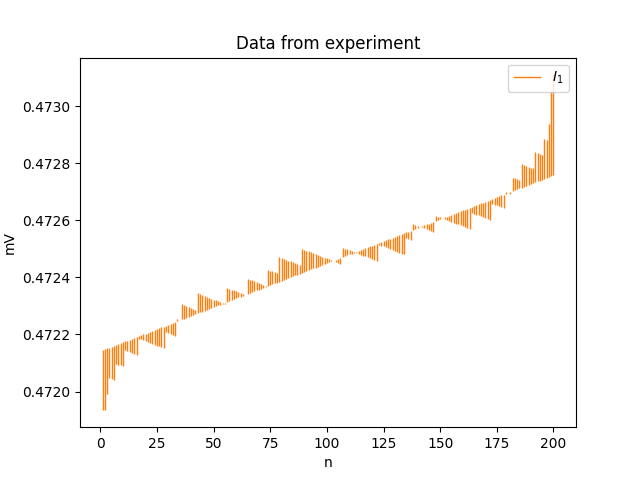
\includegraphics[width=15cm]{pics/input.png}
    \caption{График входных интервальных данных}
    \label{fig:input}
\end{figure}

\begin{figure}[H]
    \centering
    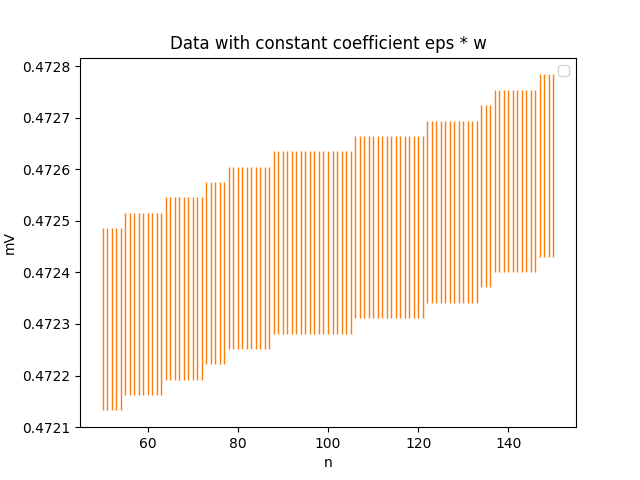
\includegraphics[width=15cm]{pics/max_w.png}
    \caption{График входных интервальных данных, с радиусом равным max($w_i$)}
    \label{fig:max_w}
\end{figure}

\begin{figure}[H]
    \centering
    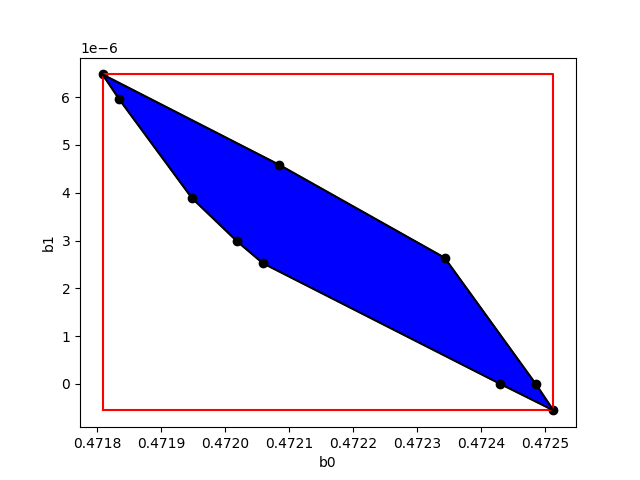
\includegraphics[width=12cm]{pics/I.png}
    \caption{Информационное множество}
    \label{fig:I}
\end{figure}

\begin{figure}[H]
    \centering
    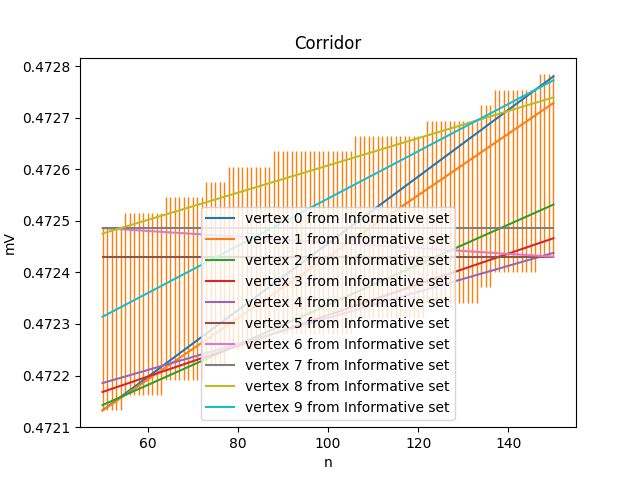
\includegraphics[width=12cm]{pics/corridor.png}
    \caption{Допусковый корридор}
    \label{fig:corridor}
\end{figure}

\begin{figure}[H]
    \centering
    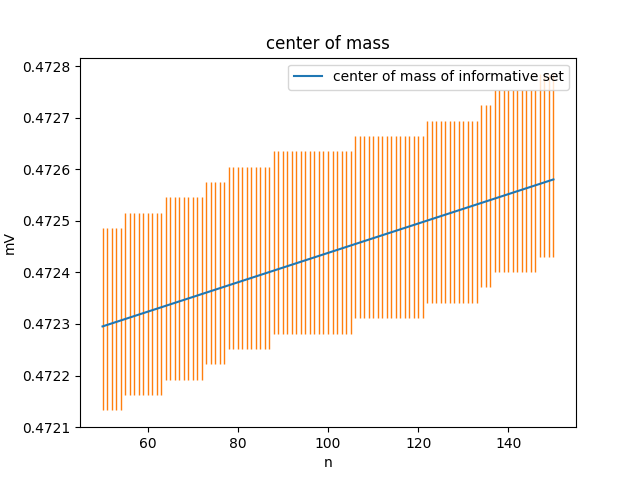
\includegraphics[width=12cm]{pics/center_of_mass.png}
    \caption{Прямая заданная центом масс информационного множества параметров}
    \label{fig:center_of_mass}
\end{figure}

\begin{figure}[H]
    \centering
    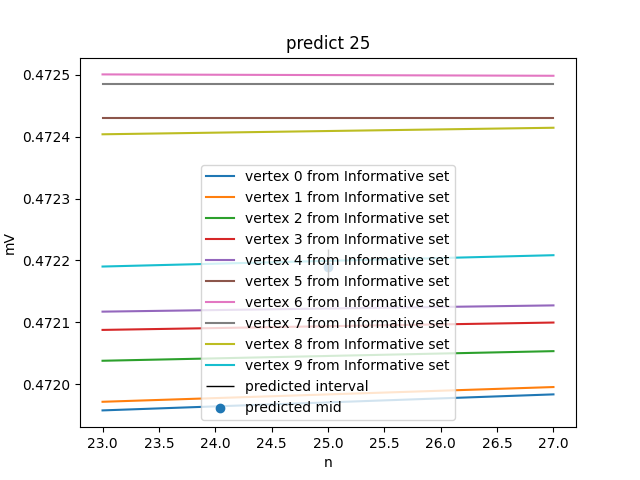
\includegraphics[width=12cm]{pics/predict25.png}
    \caption{Предсказание значения при аргументе 25}
    \label{fig:predict101.5}
\end{figure}

\begin{figure}[H]
    \centering
    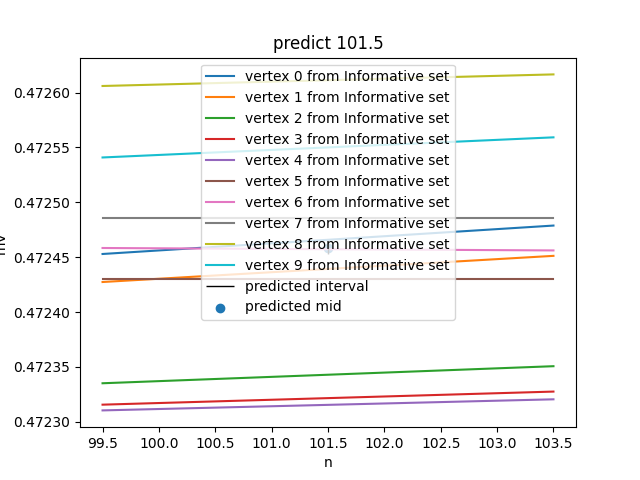
\includegraphics[width=12cm]{pics/predict101.5.png}
    \caption{Предсказание значения при аргументе 101.5}
    \label{fig:predict-10}
\end{figure}

\begin{figure}[H]
    \centering
    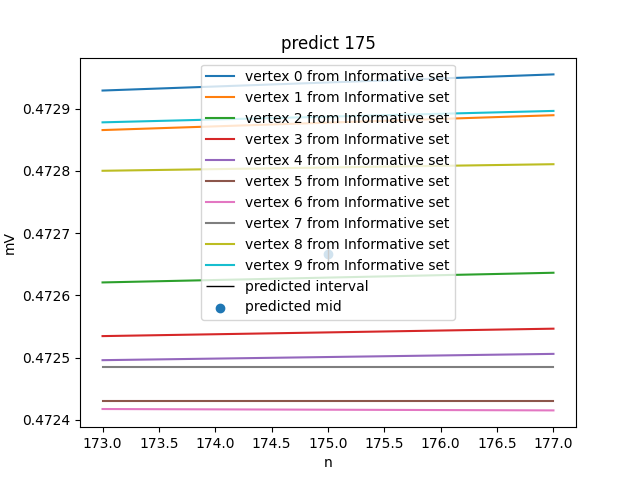
\includegraphics[width=12cm]{pics/predict175.png}
    \caption{Предсказание значения при аргументе 175}
    \label{fig:predict1000}
\end{figure}

\subsection{Числовые значения}
Уравнения вершин информационного множества
$$y = 0.4719483723913043 + 3.88695652173988e-06 * x$$
$$y = 0.47251358999999993 + -5.548999999993587e-07 * x$$
$$y = 0.47180855812500005 + 6.4759374999995055e-06 * x$$
$$y = 0.47183435499999976 + 5.960000000004851e-06 * x$$
$$y = 0.47201911500000027 + 2.979999999996874e-06 * x$$
$$y = 0.47248584499999996 + 0.0 * x$$
$$y = 0.4720846911538462 + 4.584615384614845e-06 * x$$
$$y = 0.47205911771186443 + 2.525423728813733e-06 * x$$
$$y = 0.4723432576582278 + 2.640506329113965e-06 * x$$
$$y = 0.472430355 + 0.0 * x$$
Уравнение прямой задаваемой центром масс информационного множества
$$y = 0.47215272570402433 + 2.849853946428429e-06 * x$$
Уравнение прямой полученной в результате минимизации по всей выборке
$$y = 0.472144686 + 3.0827587939700156e-06 * x$$
Предсказанные значения
$$y(25) = [0.47197045656250003, 0.47249971749999997]$$
$$mid = 0.47223508703125, rad = 0.0002646304687499712$$


$$y(101.5) = [0.472315448220339, 0.4726112690506329]$$
$$mid = 0.47246335863548594, rad = 0.0001479104151469457$$


$$y(175) = [0.4724164825, 0.4729418471875]$$
$$mid = 0.47267916484375, rad = 0.000262682343749987$$
Истинные значения
$$y(25) = [0.4721611276, 0.4722186724]$$
$$mid = 0.4721899, rad = 2.877239999998782e-05$$
$$JK = 0.1087267091196994$$


$$y(101.5) = [0.47245296207, 0.47246323793]$$
$$mid = 0.4724581, rad = 5.137930000009838e-06$$
$$JK = 0.03473676951623332$$


$$y(175) = [0.4726523138, 0.4726810862]$$
$$mid = 0.4726667, rad = 1.438619999999391e-05$$
$$JK = 0.05476652825089094$$

\section{Обсуждение}
\begin{enumerate}
    \item Исходя из предсказанных значений можно заметить, что при экстраполяции радиус гораздо больше чем при интерполяции.
    \item Спрогнозированные значения и реальные значения для рассмотренных элементов выборки являются совместными, о чем говорит положительный коэффициент Жаккара.
\end{enumerate}
\end{document}
